% !TEX root = main.tex

\chapter{はじめに}

% 多次元索引の概要・有用性
多次元索引は複数の次元で表されたキーによる検索を補助するデータ構造である.
地理情報システムにおける空間オブジェクトの検索や,データベース管理システムにおける多次元データの選択演算効率化などに利用される.
多次元データは複数の次元から成るが,メモリやストレージ上では1次元空間上に配置されるため,多次元空間上での局所性を適切に反映した索引構造が求められる.

% 多次元索引の種類
多次元索引は多次元空間を直接扱うものと1次元空間へ射影して扱うものの大きく2つに分けられ,本稿では後者を主に扱う.
多次元空間を直接扱う索引の代表例はR木~\cite{sigmod:Beckmann1990}であり,多次元のバウンディングボックスなどを用いて多次元空間を階層的に分割していく.
1次元空間へ射影するものは主に空間充填曲線に基づいており,Universal B木(UB木)~\cite{wwca:Bayer1997}が代表である.
後者の利点は,既存の効率的な1次元索引を流用でき,挿入・削除に伴う木の構造変更などが容易な点である.
一方で欠点として,多次元データを1次元化するため,隣接するデータが多次元空間上では近接していない可能性がある点が挙げられる.

% UARTの提案と問題点
本稿ではUB木およびAdaptive Radix Tree(ART)~\cite{icde:Leis2013}を組み合せた索引構造であるUniversal ART(UART)~\cite{deim:Suzuki2023}の改善について述べる.
UARTは汎用的に使用可能な多次元索引だが,データに偏りがある場合に挿入と範囲検索の性能が低下するという課題を持つ.
性能低下の原因は,不適切な空間分割による疎な部分空間の生成である.
UARTではノードの空きスペースがなくなった際に対応する多次元空間を分割することでノードを分割するが,分割後の部分空間が十分な数のレコードを持つという保証がない.
そのため挿入されるレコードに空間的な偏りがある際に,レコードを少数しか持たない疎なノードが多数生成され性能を低下させている.

% 本論文の目的と論文構成
本研究では分割後の各空間が十分な数のレコードを持つよう空間分割の手法を改善する.
まず,UARTの基となるARTとUB木の概要について述べ,続けてUARTの概要について述べる.
最後に,既存手法における空間分割の問題点と空間使用量に基づく空間分割の改善について説明し,論文全体のまとめを述べる.




\chapter{関連研究}

UARTの構成要素として利用するUB木とARTについて説明する.

\section{Universal B Tree(UB木)}

UB木~\cite{wwca:Bayer1997}は,多次元空間をZ階数曲線に基づき一次元空間に変換し,変換後のZ値を\BTree{}のキーとして使用する索引構造である.

\subsection{Z値}

Z階数曲線~\cite{acm:Gaede1998}は空間充填曲線の一種であり,二次元空間であれば``Z''の記号を描くような曲線となる.
Z値はZ階数曲線上の開始点からの距離であり,距離が近いものは多次元空間上でも近いことが多い.
ただし,空間充填曲線の性質上,Z値としては隣接するものが多次元空間上では遠く離れる場合もある.
Z値への変換は,多次元座標の各座標を2進符号化し上位ビットから順に交互配置することで行う.

\subsection{\BTree{}}
\BTree{}~\cite{book:Kitagawa1996}は,

\subsection{空間分割}

UB木は\BTree{}の一種であるためそのデータ構造は効率的だが,空間分割が非効率的であるという問題がある.
UB木はノードの空き容量がなくなった際にノードを分割するが,分割点は分割後のサイズによって決定され,空間的な面は基本的に考慮されない.
つまり,多次元空間上で非連続な領域が同じノードに割り当てられる可能性があり,各ノードに対応する多次元バウンディングボックスが過剰に拡大しうる.

\section{Adaptive Radix Tree(ART)}

ART~\cite{icde:Leis2013}は基数木(Radix Tree)の拡張であり,レコード数に応じてノードサイズを動的に選択する索引構造である.

\subsection{基数木(Radix Tree)}

\subsection{ノードサイズ}

ARTでは与えられたキーを1バイトの部分キーに分割し索引を構築するため,各ノードで最大256個のレコードを保持する.
選択されるノードはNode4,Node16,Node48,Node256の4種類であり,それぞれ対応する数のレコードを格納できる.

\subsection{空間分割}

つまり,部分キーに偏りのある箇所では容量の少ないノードが使用され,基数木の欠点である空間利用効率の悪化を克服している.





\chapter{Universal Adaptive Radix Tree(UART)}

UARTはUB木を拡張し,主に空間分割を担うART層と挿入されたレコードの保持を担うUB層に分けた多次元索引である.
Z階数曲線は多次元空間を一次元上の値として表現しており,上位ビットから下位ビットに進むにつれ粒度の細かい空間分割が行われる.
そこで,UARTでは変換後のZ値を1バイトずつの部分キーに区切り,部分キーによって表される空間分割をARTにより管理する.
つまり,ART層では多次元空間上でレコードが密な領域ほど空間が分割され,深い階層が生成される.
UB層は挿入されたレコードを保持するデータ層であり,該当領域に存在する疎なレコード群への効率的な範囲走査を実現する.

\Fig{\ref{fig:uart}}にUARTの概念図を示す.
本来のUARTではZ値を1バイトずつに区切るが,\Fig{\ref{fig:uart}}ではZ値を4ビットごとに区切っている.
また,ART層の丸はレコードを,UB層の丸はUB木のノードを表している.
そして,区切られたZ値のうち上位4ビットと中位4ビットはそれぞれの層のグレー色に塗りつぶされた区画に,下位の4ビットは最下層の灰色のレコードに対応している.
以下では,ART層とUB層の構造について概略を述べる.

\begin{figure}[t]
  \centering
  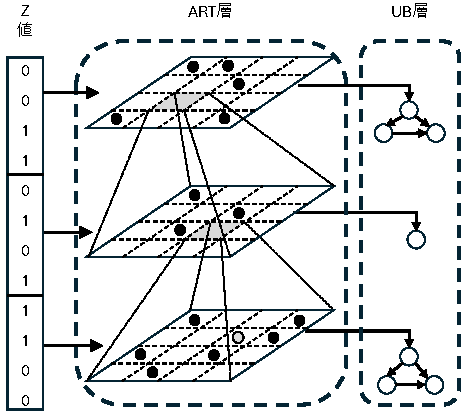
\includegraphics{./figures/fig_uart.pdf}
  \caption{UARTの構造}
  \label{fig:uart}
\end{figure}

\paragraph{ART層}

ART層はZ値をキーとしてARTに格納することで多次元空間を階層的に分割する索引層である.
ARTではキーを1バイトの部分キーに分割するため,各階層で空間は256分割される.
分割された空間のうちレコードが密に存在する箇所は後述する手続きによって下の階層が生成され,再帰的により細かい空間分割が行われる.
一方,ART中の各ノードはUB木の根ノード(i.e., UB層へのポインタ)をヘッダ領域に持ち,下の階層を持たない空間のレコードはそちらで保持される.

\paragraph{UB層}

UB層はART層の各階層各空間で保持されるUB木の集合であり,レコードの実体はこちらで管理される.
各UB木はその階層におけるZ値の部分キーを検索キー,挿入された空間オブジェクトとペイロードの組をレコードとして持つ.
なお最下層,つまりZ値の全長を用いた空間分割後のUB木は,部分キーとなるZ値を持たないため一般的な\BTree{}として生成される.
UB木の構築方法は既存のものと同様であり,\BTree{}に由来する効率的な範囲走査を可能とする.
ただし,既存研究において各UB木は根ノードのみしか持たない点に注意する~\cite{deim:Suzuki2023}.





\chapter{UARTにおける空間分割の効率化}

既存研究の課題として,オブジェクトが疎に分布する空間の管理が不十分であり,偏った分布における性能低下が挙げられる~\cite{deim:Suzuki2023}.
例えば全オブジェクトが1つの部分空間に偏る場合は,最下層までARTが展開され,\BTree{}によって全オブジェクトが管理されるため空間効率に関する問題は発生しない.
同様に,オブジェクトが空間全域で一様に分布する場合は,各部分空間に対応するUB木が一定数のオブジェクトを管理するためこちらも問題ない.
しかし,分布が適度に偏っているとき,既存のUARTでは少数のレコードしか持たないUB木が多数生成され性能が低下してしまう.

分布の偏りによる性能低下は,既存研究におけるUB木が根ノード1つしか持たず,オブジェクトが疎な空間のレコードを十分に保持できないためである.
既存研究ではUB木の根ノードを一種の書込み用バッファとして利用しており,空き容量がなくなった際は即座にオブジェクト数が最も多い部分空間を選びART層で下層を生成する.
この密な空間を選ぶという方針自体は誤っていないが,部分空間における空間使用量を考慮せず,単純にレコード数の多い空間を選ぶという手続きに問題がある.
つまり,各部分空間のオブジェクト数の差が少ない(i.e., 分布がロングテールを持つ)とき,この手続きではオブジェクト数が少ない部分空間においても下層が生成されてしまう.
現実的なワークロードやデータセットにおいてロングテールは頻出するため,この問題への対応は必須である.

そこで本研究では,下層生成の条件として一定の空間使用量を持つことを使用し,UB層において根ノード単体ではなくUB木としてレコードを保持する.
UB木はZ値を使用した二次索引であり,同じZ値を持つレコードは内部で転置リスト(posting list)として保持される.
既存研究では各転置リスト内のレコード数のみを見たが,本研究では転置リストのサイズも考慮し一定のサイズを超えるまで下層を生成しない.
つまり,ノードの空き容量がなく下層も生成しない場合はノードを分割し,UB木を拡張する.
これにより,生成された下層には一定以上のオブジェクトが必ず含まれるため,各ノードの空間利用効率およびそれに伴う範囲走査性能の向上が見込める.





\chapter{評価実験}






\chapter{おわりに}

本研究では,UARTにおける空間分割の効率化によるメモリ利用効率の向上について提案した.
空間使用量を考慮していないという既存研究の課題について説明し,UARTにおける空間使用量を考慮した空間分割について述べた.
今後は提案手法の実装,および既存研究との比較による有効性の検証を行う予定である.





\chapter*{謝辞}

本研究の一部はJSPS科研費JP20K19804,JP21H03555,JP22H03594の助成,日本電信電話株式会社との共同研究,および国立研究開発法人新エネルギー・産業技術総合開発機構(NEDO)の委託業務(JPNP16007)の結果得られたものである.